%%
%% This is file `sample-manuscript.tex',
%% generated with the docstrip utility.
%%
%% The original source files were:
%%
%% samples.dtx  (with options: `all,proceedings,bibtex,manuscript')
%%
%% IMPORTANT NOTICE:
%%
%% For the copyright see the source file.
%%
%% Any modified versions of this file must be renamed
%% with new filenames distinct from sample-manuscript.tex.
%%
%% For distribution of the original source see the terms
%% for copying and modification in the file samples.dtx.
%%
%% This generated file may be distributed as long as the
%% original source files, as listed above, are part of the
%% same distribution. (The sources need not necessarily be
%% in the same archive or directory.)
%%
%%
%% Commands for TeXCount
%TC:macro \cite [option:text,text]
%TC:macro \citep [option:text,text]
%TC:macro \citet [option:text,text]
%TC:envir table 0 1
%TC:envir table* 0 1
%TC:envir tabular [ignore] word
%TC:envir displaymath 0 word
%TC:envir math 0 word
%TC:envir comment 0 0
%%
%%
%% The first command in your LaTeX source must be the \documentclass
%% command.
%%
%% For submission and review of your manuscript please change the
%% command to \documentclass[manuscript, screen, review]{acmart}.
%%
%% When submitting camera ready or to TAPS, please change the command
%% to \documentclass[sigconf]{acmart} or whichever template is required
%% for your publication.
%%
%%
% \documentclass[manuscript,screen,review,anonymous]{acmart}
\documentclass[acmsmall,sigconf]{acmart}

%%
%% \BibTeX command to typeset BibTeX logo in the docs
\AtBeginDocument{%
  \providecommand\BibTeX{{%
    Bib\TeX}}}

% %% Rights management information.  This information is sent to you
% %% when you complete the rights form.  These commands have SAMPLE
% %% values in them; it is your responsibility as an author to replace
% %% the commands and values with those provided to you when you
% %% complete the rights form.
% \setcopyright{acmlicensed}
% \copyrightyear{2018}
% \acmYear{2018}
% \acmDOI{XXXXXXX.XXXXXXX}

% %% These commands are for a PROCEEDINGS abstract or paper.
% \acmConference[Conference acronym 'XX]{Make sure to enter the correct
%   conference title from your rights confirmation emai}{June 03--05,
%   2018}{Woodstock, NY}
% %%
% %%  Uncomment \acmBooktitle if the title of the proceedings is different
% %%  from ``Proceedings of ...''!
% %%
% %%\acmBooktitle{Woodstock '18: ACM Symposium on Neural Gaze Detection,
% %%  June 03--05, 2018, Woodstock, NY}
% \acmISBN{978-1-4503-XXXX-X/18/06}


%%
%% Submission ID.
%% Use this when submitting an article to a sponsored event. You'll
%% receive a unique submission ID from the organizers
%% of the event, and this ID should be used as the parameter to this command.
%%\acmSubmissionID{123-A56-BU3}

%%
%% For managing citations, it is recommended to use bibliography
%% files in BibTeX format.
%%
%% You can then either use BibTeX with the ACM-Reference-Format style,
%% or BibLaTeX with the acmnumeric or acmauthoryear sytles, that include
%% support for advanced citation of software artefact from the
%% biblatex-software package, also separately available on CTAN.
%%
%% Look at the sample-*-biblatex.tex files for templates showcasing
%% the biblatex styles.
%%

%%
%% The majority of ACM publications use numbered citations and
%% references.  The command \citestyle{authoryear} switches to the
%% "author year" style.
%%
%% If you are preparing content for an event
%% sponsored by ACM SIGGRAPH, you must use the "author year" style of
%% citations and references.
%% Uncommenting
%% the next command will enable that style.
%%\citestyle{acmauthoryear}

\usepackage{mathtools}
\usepackage{multirow}
\usepackage{subcaption}

\graphicspath{{images/}}
\DeclareGraphicsExtensions{.pdf}

\DeclarePairedDelimiter{\set}{\{}{\}}
\DeclarePairedDelimiter{\tuple}{(}{)}
\DeclarePairedDelimiter{\abs}{\lvert}{\rvert}
\renewcommand{\implies}{\rightarrow}
\newcommand{\db}{D}
\newcommand{\dbs}{\mathcal{D}}
\newcommand{\model}{\mathcal{M}}
\newcommand{\priv}{R}
\newcommand{\pos}{\hat{P}}
\newcommand{\posm}{\hat{P}_\mathcal{M}}
\newcommand{\tru}{T}
\newcommand{\leg}{L}
\newcommand{\sco}{\hat{S}}
\newcommand{\scom}{\hat{S}_\mathcal{M}}
\newcommand{\calib}{C}
\newcommand{\prob}[1]{\text{Pr}[#1]}

%%
%% end of the preamble, start of the body of the document source.
\begin{document}

%%
%% The "title" command has an optional parameter,
%% allowing the author to define a "short title" to be used in page headers.
\title{The Name of the Title Is Hope}

%%
%% The "author" command and its associated commands are used to define
%% the authors and their affiliations.
%% Of note is the shared affiliation of the first two authors, and the
%% "authornote" and "authornotemark" commands
%% used to denote shared contribution to the research.
\author{Chih-Cheng Rex Yuan}
\email{hello@rexyuan.com}
\affiliation{%
  \institution{Institute of Information Science, Academia Sinica}
  \city{Taipei}
  \country{Taiwan}
}

\author{Bow-Yaw Wang}
\email{bywang@iis.sinica.edu.tw}
\affiliation{%
  \institution{Institute of Information Science, Academia Sinica}
  \city{Taipei}
  \country{Taiwan}
}

%%
%% By default, the full list of authors will be used in the page
%% headers. Often, this list is too long, and will overlap
%% other information printed in the page headers. This command allows
%% the author to define a more concise list
%% of authors' names for this purpose.
% \renewcommand{\shortauthors}{Trovato et al.}

%%
%% The abstract is a short summary of the work to be presented in the
%% article.
\begin{abstract}
  abstract
\end{abstract}

% %%
% %% The code below is generated by the tool at http://dl.acm.org/ccs.cfm.
% %% Please copy and paste the code instead of the example below.
% %%
% \begin{CCSXML}
% <ccs2012>
%  <concept>
%   <concept_id>00000000.0000000.0000000</concept_id>
%   <concept_desc>Do Not Use This Code, Generate the Correct Terms for Your Paper</concept_desc>
%   <concept_significance>500</concept_significance>
%  </concept>
%  <concept>
%   <concept_id>00000000.00000000.00000000</concept_id>
%   <concept_desc>Do Not Use This Code, Generate the Correct Terms for Your Paper</concept_desc>
%   <concept_significance>300</concept_significance>
%  </concept>
%  <concept>
%   <concept_id>00000000.00000000.00000000</concept_id>
%   <concept_desc>Do Not Use This Code, Generate the Correct Terms for Your Paper</concept_desc>
%   <concept_significance>100</concept_significance>
%  </concept>
%  <concept>
%   <concept_id>00000000.00000000.00000000</concept_id>
%   <concept_desc>Do Not Use This Code, Generate the Correct Terms for Your Paper</concept_desc>
%   <concept_significance>100</concept_significance>
%  </concept>
% </ccs2012>
% \end{CCSXML}

% \ccsdesc[500]{Do Not Use This Code~Generate the Correct Terms for Your Paper}
% \ccsdesc[300]{Do Not Use This Code~Generate the Correct Terms for Your Paper}
% \ccsdesc{Do Not Use This Code~Generate the Correct Terms for Your Paper}
% \ccsdesc[100]{Do Not Use This Code~Generate the Correct Terms for Your Paper}

% %%
% %% Keywords. The author(s) should pick words that accurately describe
% %% the work being presented. Separate the keywords with commas.
% \keywords{Do, Not, Us, This, Code, Put, the, Correct, Terms, for,
%   Your, Paper}

\received{20 February 2007}
\received[revised]{12 March 2009}
\received[accepted]{5 June 2009}

%%
%% This command processes the author and affiliation and title
%% information and builds the first part of the formatted document.
\maketitle

\section{Introduction}

\section{Related Work}

\clearpage

\section{Preliminaries}

A \emph{row} $r_i$ is a lookup table or dictionary. A \emph{database} $\db = \set{r_1, r_2, ...}$ is a collection of rows. The set of all databases is denoted $\dbs$. The attributes of a $\db$ is $\mathcal{A} = \set{A_1, A_2, ...}$. The domain of $A_i$ is $\Omega_i$.

\subsection{Fairness Measures}

For fairness measures\cite{yuan2024ensuring,pessach2022review}, let $Y$ to denote the ground truth of an outcome, let $\hat{Y}$ to denote the predicated result of an outcome, let $S$ denote the protected attribute, and let $\epsilon$ denote some threshold. For non-binary prediction, such as a score, we use $\hat{V}$.

Fairness measures can be broadly categorized into independence, separation, and sufficiency, which are defined by conditional independence in Table~\ref{tab:categories}.

\begin{table}[h]
\caption{Fairness categories.}
\label{tab:categories}
\begin{tabular}{cc}
\toprule
\textbf{Category} & \textbf{Definition} \\
\midrule
Independence & $S \bot \hat{Y}$ \\
Separation & $S \bot \hat{Y} | Y$ \\
Sufficiency & $S \bot Y | \hat{Y}$ \\
\bottomrule
\end{tabular}
\end{table}

These categories can be expanded into forms of probability. For example, the definition of separation is expanded to
\begin{align*}
P[\hat{Y} = 1 | S = 1, Y = 1] & = P[\hat{Y} = 1 | S \neq 1, Y = 1] \\
P[\hat{Y} = 1 | S = 1, Y = 0] & = P[\hat{Y} = 1 | S \neq 1, Y = 0]
\end{align*}
The definition can be relaxed. Its relaxation, for some parameter $\epsilon$, is
\begin{align*}
\abs{P[\hat{Y} = 1 | S = 1, Y = 1] - P[\hat{Y} = 1 | S \neq 1, Y = 1]} & \leq \epsilon \\
\abs{P[\hat{Y} = 1 | S = 1, Y = 0] - P[\hat{Y} = 1 | S \neq 1, Y = 0]} & \leq \epsilon
\end{align*}
which is also the definition of a fairness measure called equalized odds.

We consider in this work various fairness measures listed in Table~\ref{tab:measures}.

% \begin{definition}[Independence\cite{barocas2023fairness}]\label{def:independence}
% $(S, \hat{Y})$ satisfy independence if and only if $S \bot \hat{Y}$; that is
% \[
% P[\hat{Y} = 1 | S = 1] = P[\hat{Y} = 1 | S \neq 1]
% \]
% A relaxation of independence on a threshold is
% \[
% \abs{P[\hat{Y} = 1 | S = 1] - P[\hat{Y} = 1 | S \neq 1]} \leq \epsilon
% \]
% \end{definition}

% \begin{definition}[Separation\cite{barocas2023fairness}]\label{def:separation}
% $(S, Y, \hat{Y})$ satisfy separation if and only if $S \bot \hat{Y} | Y$; that is
% \begin{align*}
% P[\hat{Y} = 1 | S = 1, Y = 1] & = P[\hat{Y} = 1 | S \neq 1, Y = 1] \\
% P[\hat{Y} = 1 | S = 1, Y = 0] & = P[\hat{Y} = 1 | S \neq 1, Y = 0]
% \end{align*}
% A relaxation of independence on a threshold is
% \begin{align*}
% \abs{P[\hat{Y} = 1 | S = 1, Y = 1] - P[\hat{Y} = 1 | S \neq 1, Y = 1]} & \leq \epsilon \\
% \abs{P[\hat{Y} = 1 | S = 1, Y = 0] - P[\hat{Y} = 1 | S \neq 1, Y = 0]} & \leq \epsilon
% \end{align*}
% \end{definition}

% \begin{definition}[Sufficiency\cite{barocas2023fairness}]\label{def:separation}
% $(S, Y, \hat{Y})$ satisfy sufficiency if and only if $S \bot Y | \hat{Y}$; that is
% \begin{align*}
% P[Y = 1 | S = 1, \hat{Y} = 1] & = P[Y = 1 | S \neq 1, \hat{Y} = 1] \\
% P[Y = 1 | S = 1, \hat{Y} = 0] & = P[Y = 1 | S \neq 1, \hat{Y} = 0]
% \end{align*}
% A relaxation of independence on a threshold is
% \begin{align*}
% \abs{P[Y = 1 | S = 1, \hat{Y} = 1] - P[Y = 1 | S \neq 1, \hat{Y} = 1]} & \leq \epsilon \\
% \abs{P[Y = 1 | S = 1, \hat{Y} = 0] - P[Y = 1 | S \neq 1, \hat{Y} = 0]} & \leq \epsilon
% \end{align*}
% \end{definition}

% The $p$-norm is denoted by $L_p$ and the $p$-norm of a vector $x$ is denoted by $\Vert x \Vert_p$.

% The normal distribution or Gaussian distribution with mean $\mu$ and standard deviation $\sigma$ is denoted by $\mathcal{N}(\mu, \sigma^2)$.

\begin{table*}[h]
\caption{Fairness measures.}
\label{tab:measures}
\begin{tabular}{llc}
\toprule
\textbf{Category} & \textbf{Fairness Measure} & \textbf{Definition} \\
\midrule
\multirow{4}{*}{Independence} & Disparate Impact & $\frac{P[\hat{Y} = 1 | S \neq 1]}{P[\hat{Y} = 1 | S = 1]} \geq 1 - \epsilon$ \\
& Demographic Parity & $\abs{P[\hat{Y} = 1 | S = 1] - P[\hat{Y} = 1 | S \neq 1]} \leq \epsilon$ \\
& Conditional Statistical Parity & $\abs{P[\hat{Y} = 1 | S = 1, L = l] - P[\hat{Y} = 1 | S \neq 1, L = l]} \leq \epsilon$ \\
& Mean Difference & $\abs{E[\hat{Y}|S = 1] - E[\hat{Y}|S \neq 1]} \leq \epsilon$ \\
\multirow{4}{*}{Separation} & \multirow{2}{*}{Equalized Odds} & $\abs{P[\hat{Y} = 1 | S = 1, Y = 0] - P[\hat{Y} = 1 | S \neq 1, Y = 0]} \leq \epsilon$ \\
& & $\abs{P[\hat{Y} = 1 | S = 1, Y = 1] - P[\hat{Y} = 1 | S \neq 1, Y = 1]} \leq \epsilon$ \\
& Equal Opportunity & $\abs{P[\hat{Y} = 1 | S = 1, Y = 1] - P[\hat{Y} = 1 | S \neq 1, Y = 1]} \leq \epsilon$ \\
& Predictive Equality & $\abs{P[\hat{Y} = 1 | S = 1, Y = 0] - P[\hat{Y} = 1 | S \neq 1, Y = 0]} \leq \epsilon$ \\
\multirow{4}{*}{Sufficiency} & \multirow{2}{*}{Conditional Use Accuracy Equality} & $\abs{P[Y = 1 | S = 1, \hat{Y} = 1] - P[Y = 1 | S \neq 1, \hat{Y} = 1]} \leq \epsilon$ \\
& & $\abs{P[Y = 0 | S = 1, \hat{Y} = 0] - P[Y = 0 | S \neq 1, \hat{Y} = 0]} \leq \epsilon$ \\
& Predictive Parity & $\abs{P[Y = 1 | S = 1, \hat{Y} = 1] - P[Y = 1 | S \neq 1, \hat{Y} = 1]} \leq \epsilon$ \\
& Equal Calibration & $\abs{P[Y = 1 | S = 1, \hat{V} = v] - P[Y = 1 | S \neq 1, \hat{V} = v]} \leq \epsilon$ \\
\multirow{3}{*}{N/A} & Overall Accuracy Equality & $\abs{P[Y = \hat{Y} | S = 1] - P[Y = \hat{Y} | S \neq 1]} \leq \epsilon$ \\
& Positive Balance & $\abs{E[\hat{V} | Y = 1, S = 1] - E[\hat{V} | Y = 1, S \neq 1]} \leq \epsilon$ \\
& Negative Balance & $\abs{E[\hat{V} | Y = 0, S = 1] - E[\hat{V} | Y = 0, S \neq 1]} \leq \epsilon$ \\
\bottomrule
\end{tabular}
\end{table*}

\subsection{Differential Privacy}

% \begin{definition}[Sensitivity\cite{dwork2014algorithmic}]\label{def:sensitivity}
% Let $f$ be a function that takes a database $\db$ and outputs a vector $\mathbb{R}^p$. The $L_2$ sensitivity of $f$ is for all databases $\db_1,\db_2$ that differ in exactly one row:
% \[
% \Delta^2_f = max_{\db_1,\db_2} \Vert f(\db_1) - f(\db_2) \Vert_p
% \]
% \end{definition}

% \begin{definition}[Differential Privacy (DP) \cite{dwork2006calibrating,dwork2014algorithmic,mckenna2021winning}]\label{def:rdp}
% A randomized mechanism $M$ satisfies $(\epsilon,\delta)$-DP if, for all databases $\db_1,\db_2$ that differ in exactly one row and for all subsets $S$ of $R$, we have
% \[
% \prob{M(\db_1) \in S} \leq e^\epsilon \prob{M(\db_2) \in S} + \delta
% \]
% \end{definition}

A \emph{randomized mechanism} is a randomized algorithm $M : \dbs \implies R$ that takes a database and, after introducing noise, outputs some results.

\begin{definition}[Gaussian Mechanism\cite{dwork2014algorithmic}]\label{def:gm}
Let $f : \dbs \implies \mathbb{R}^p$ be a function that takes a database and outputs a vector. The Gaussian Mechanism $M$ adds i.i.d. Gaussian noise with scale $\sigma$ to each of the $p$ outputs:
\[
M(\db) = f(\db) + \mathcal{N}(0, \sigma^2 \mathbb{I})
\]
\end{definition}

\begin{definition}[R\'enyi Differential Privacy (RDP)]\label{def:rdp}
A randomized mechanism $M$ satisfies $(\alpha,\gamma)$-RDP for $\alpha \geq 1$ and $\gamma \geq 1$ if, for all databases $\db_1,\db_2$ that differ in exactly one row, we have
\[
D_\alpha(M(\db_1) \Vert M(\db_2)) \leq \gamma
\]
where $D_\alpha$ is the R\'enyi divergence\cite{van2014renyi} of order $\alpha$.
\end{definition}

\begin{theorem}[RDP of the Gaussian Mechanism\cite{feldman2018privacy,mironov2017renyi}]
The Gaussian Mechanism satisfies $(\alpha, \alpha \frac{\Delta^2_f}{2 \sigma^2})$-RDP.
\end{theorem}

\subsection{Differentially Private Synthetic Data}

Let $C \subseteq \mathcal{A}$ be a subset of attributes. Let $\Omega_C = \Pi_{i \in C} \Omega_i$. A \emph{marginal}\cite{barak2007privacy,mckenna2021winning} of $C$ is a vector $\mu \in \mathbb{R}^{\abs{\Omega_C}}$, indexed by domain element $t \in \Omega_C$, such that each entry is a count $\mu_t = \Sigma_{x \in \db} \vmathbb{1} [x_C = t]$ where $\vmathbb{1}$ is the indicator function; that is, it is the vector of the count of each possible element.

Let $M_C(\db)$ be the function that computes the marginal of $C$ on $\db$, i.e., $\mu = M_C(\db)$. We call marginals of $|C| = n$ attributes $n$-way marginals.

The task of differentially private synthetic data is, given a database $\db$, adding some noise such that it satisfies differential privacy guarantee and outputting another database $\db'$, such that the $L_1$ errors between some selected marginals $C_1,C_2,...$ of $\db$ and $\db'$ is small; that is, their marginals $(M_{C_1}(\db),M_{C_1}(\db')),(M_{C_2}(\db),M_{C_2}(\db')),...$ are similar.

For example, suppose we have a database with attributes sex and race. The 2-way marginals of the original database and the synthetic database are shown in Table~\ref{tab:marginal-example}. The marginals of the synthetic data is supposed to be similar to that of the original database.

\begin{table}[h]
\caption{Example marginals.}
\label{tab:marginal-example}
\centering
\begin{subtable}[t]{0.45\linewidth}
\centering
\caption{Marginal of original data.}
\begin{tabular}{cc}
\toprule
Attributes & Count \\
\midrule
Male,White & 24 \\
Female,White & 33 \\
Male,Black & 13 \\
Female,Black & 47 \\
\bottomrule
\end{tabular}
\end{subtable}
\hspace{0.05\linewidth}
\begin{subtable}[t]{0.45\linewidth}
\centering
\caption{Marginal of synthetic data.}
\begin{tabular}{cc}
\toprule
Attributes & Count \\
\midrule
Male,White & 22 \\
Female,White & 35 \\
Male,Black & 10 \\
Female,Black & 46 \\
\bottomrule
\end{tabular}
\end{subtable}
\end{table}

\section{Auditing Framework}

Our auditing framework is tripartite. It consists of three parties: the data provider, the model maker, and the third-party auditor.

The data provider is responsible for supplying the raw datasets which should originate from trustworthy sources, such as government agencies like a census bureau.

The model maker develops AI models. These are AI companies or research labs specialized in training and optimizing AI models.

The third-party auditor acts as an evaluator, using our framework to audit the AI models for fairness issues by combining both the datasets and the models. These may be investigative journalists or regulatory bodies.

In the framework of our previous work\cite{yuan2024ensuring}, after obtaining real data from the data provider, the 3rd party auditor holds onto the real data for performing fairness audits, and it supposedly retains it indefinitely for the possibility of any future audits.

However, this practice introduces security concerns. It creates a vulnerability to data security threats. A breach at the auditor's end could result in compromises of individuals' privacy.

Moreover, the storage of the datasets also raises privacy concerns. Holding large amounts of sensitive data for an extended period opens the door to the risk of misuse. The auditor may misuse the data for unauthorized purposes.

Thus, we introduce a new framework where the auditor generates synthetic data based on real data upon retrieval of the real data, and then holds onto the synthetic data and discards the real data, preventing further privacy breaches.

\section{Methodology}

We employed the tools of the winner of the 2018 NIST Differential Privacy Synthetic Data Challenge competition\cite{NIST2018} by Ryan McKenna\cite{Ullman2022,McKenna2022,McKenna_privatePGM,mckenna2021winning,mckenna2019graphical} and the fairness checker tool from our previous research\cite{yuan2024ensuring}.

This research is implemented in Python Jupyter notebooks and is publicly available.

\subsection{Data Synthesis}

The synthesis framework is three-fold, namely, select-measure-generate\cite{McKenna2022}. We first select the important marginals to preserve, measure them by adding differentially private noise, and then generate synthetic data.

Underneath the hood, the tool employs a Markov random field. The select step corresponds to marking cliques in a Markov random field, and the generate step corresponds to sampling from the fitted Markov random field.

By default, all $1$-way marginals are selected to preserve the quantity of each attribute element. We can further preserve correlations by adding $n$-way marginals. For example, if we want to preserve the relationship between sex and race, we may add the clique (sex,race).

In a perfect world where all correlation information is to be preserved, we may wish to make a completely connected graph. However, this was found to be intractable as the complexity of the problem would skyrocket.

To circumvent the complexity explosion, instead, Ryan McKenna devised a technique where the mutual information of all the database attribute pairs is calculated, and then a maximum spanning tree algorithm was run with edge weights being the mutual information to obtain a skeleton spanning-tree-shaped Markov random field.

For the competition, Ryan McKenna further manually added certain cliques based on his investigation of the competition dataset. For example, he manually added the clique (sex,city,income). In addition, he would add some edges based on some sophisticated heuristics tailored to that particular dataset.

We developed an alternative heuristic for a general-purpose workflow. From the definition of mutual information, we can obtain that they are bounded by the pair's respective Shannon entropy. Using this property, we add additional edges with weights exceeding a fraction of the minimum of these upper bounds. As a rule of thumb, we have found setting the fraction to be $0.1$ to be effective.

For the measure step, we followed the examples provided in the tool's repository. Gaussian noises are added to the selected marginals. Half of the privacy budget is spent on all 1-way marginals and the other half on the selected cliques. These marginals are then fed to the tool to fit the Markov random field. By \cite{mckenna2021winning}, this procedure satisfies $(\alpha,\frac{\alpha}{2 \sigma^2})$-RDP for all $\alpha \geq 1$.

\subsection{Fairness Checking}

After synthesizing datasets, we used the fairness checker from \cite{yuan2024ensuring} to compute their fairness measures. To test the viability of our method, we compare the metrics computed from the synthetic dataset against those of the original dataset. We used various datasets with fairness concerns mentioned in \cite{pessach2022review}.

The fairness checker evaluates datasets based on multiple fairness metrics, such as demographic parity and equalized odds. These metrics are computed on some sensitive attributes, predicted outcomes, and ground truths. Examples of sensitive attributes are race and sex. Examples of predicted outcomes and ground truths are loan approval and criminal recidivism.

By comparing these measures between the synthetic and original datasets, we aim to ensure that the synthetic data preserves the fairness properties of the original data. The comparison process is three-fold. It goes as follows.

The dataset is first processed so it can be fed into the synthetic data generator. Some marginals are selected as described in the previous section, and the synthetic data generator model is fitted to the original data according to the marginals. Then the generator is run multiple times to obtain multiple sets of synthetic data.

Next, several AI models are extracted from various real life authors from Kaggle. They are finetuned to perform well on the original dataset. For one, a random forest model is finetuned by searching hyperparameters settings\cite{Ipbyrne2023}. For another, a logistic regression model is finetuned by performing principal component analysis\cite{Prashant1112023}.

Several AI models and both the original dataset and the rounds of synthetic datasets are fed to the fairness checker. Sensitive attributes are identified based on manual examination with common sense or by referring to \cite{pessach2022review}. Then, all applicable fairness measures are computed using the checker for both the original and the synthetic.

Finally, we analyze the discrepancies between the fairness properties of the original and the synthetic by calculating the difference and the ratio of their perspective fairness measure values. The sum of the difference and the average of the ratio serve as a summary of the analysis.

\section{Results}

We looked at several publicly available datasets, such as adult\cite{adult_2,Kaggle_Adult_Census_Income}, COMPAS\cite{larson2016propublica,Kaggle_COMPAS_Dataset}, and diabetes\cite{diabetes_34,Kaggle_Diabetes_Prediction}. The adult dataset comes from the 1994 census in the United States. The COMPAS dataset comes from an investigative report by ProPublica of the COMPAS criminal recidivism assessment system. The diabetes dataset comes from the hospital readmission data published in the 1994 AI in Medicine journal.

\subsection{Adult Income Dataset}

For the adult income dataset, the shape of the maximum spanning tree is very shallow, almost resembling a star; it has one internal node and all but one of the leaves have a depth of one. After introducing edges according to our heuristic, we observed an increase in the pairwise edges of the leaves, forming many 3-cliques and two 4-cliques. The resulting graph is shown in Figure~\ref{fig:adult_mst}.

Marginals based on this graph are then passed to the synthetic data generator for model fitting.

\begin{figure}[h]
\centering
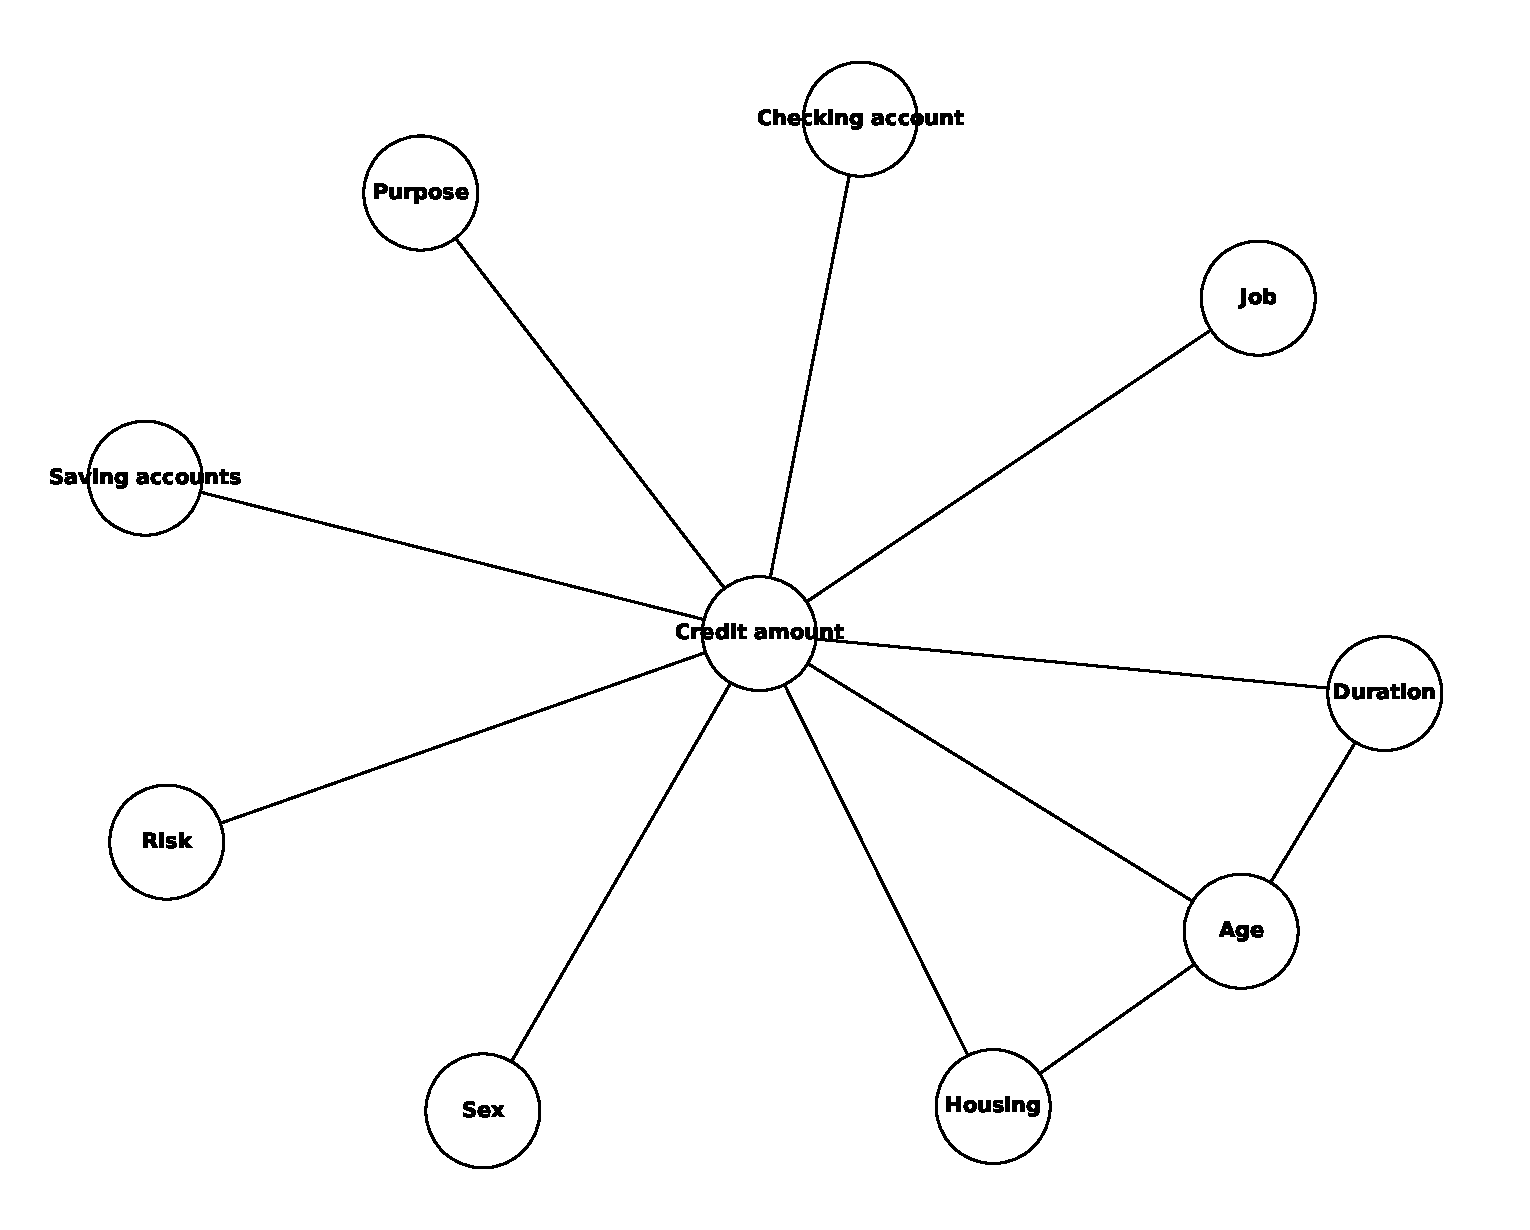
\includegraphics[width=\linewidth]{adult_mst}
\caption{Markov random field for marginals of the adult dataset.}
\label{fig:adult_mst}
\Description{Markov random field for marginals of the adult dataset.}
\end{figure}

After generating ten rounds of synthetic data and passing them to the checker, their fairness measure values are averaged. Then, we compare them against the values of the original data. The results are shown in Table~\ref{tab:adult_score}.

We observed that across all examined fairness measures, their difference all fall below 0.1. The sum of their differences is 0.259 and the average of their ratios is 0.952, which we consider quite satisfactory.

\begin{table}[h]
\caption{Fairness measures experiment results of the adult dataset. Sum of differences is 0.259. Average of ratios is 0.952.}
\label{tab:adult_score}
\begin{tabular}{ccccc}
\toprule
\textbf{Measure} & \textbf{Original} & \textbf{Synthetic} & \textbf{Diff} & \textbf{Ratio} \\
\midrule
Demographic Parity  & 0.172 & 0.104 & 0.067 & 1.651 \\
Accuracy Eqaulity   & 0.047 & 0.117 & 0.069 & 0.404 \\
Equalized Odds 1    & 0.057 & 0.079 & 0.021 & 0.723 \\
Equalized Odds 2    & 0.166 & 0.122 & 0.044 & 1.365 \\
Accuracy Equality 1 & 0.100 & 0.132 & 0.031 & 0.759 \\
Accuracy Equality 2 & 0.119 & 0.146 & 0.027 & 0.814 \\
\bottomrule
\end{tabular}
\end{table}

\subsection{COMPAS Dataset}

For the COMPAS dataset, the initial spanning tree has a long tail, which is not surprising because, upon closer inspection, they all are related to the original COMPAS risk scores. The heuristic edge addition did not change the graph significantly. It only introduced one 3-clique triangle. The resulting graph is shown in Figure~\ref{fig:compas_mst}.

Marginals of this graph are then too passed to the synthetic data generator for fitting.

\begin{figure}[h]
\centering
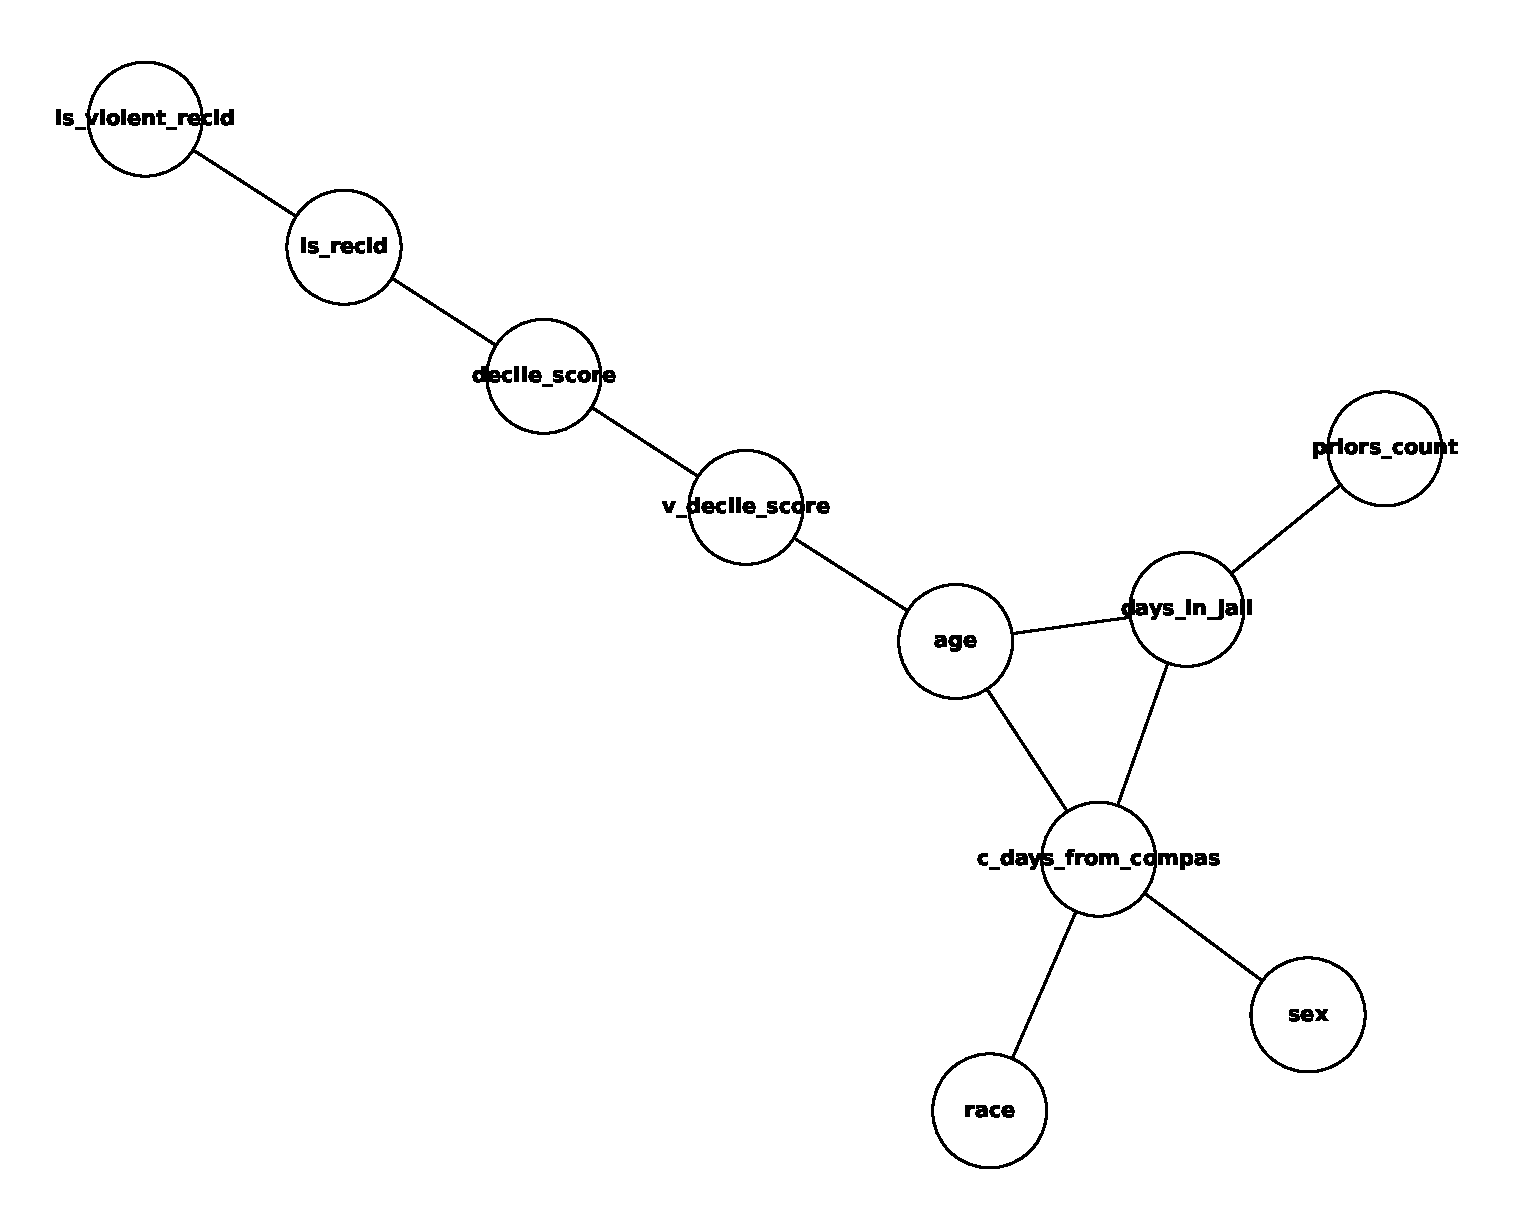
\includegraphics[width=\linewidth]{compas_mst}
\caption{Markov random field for marginals of the COMPAS dataset.}
\label{fig:compas_mst}
\Description{Markov random field for marginals of the COMPAS dataset.}
\end{figure}

We ran the same workflow as adult dataset for the COMPAS dataset. The comparison results are shown in Table~\ref{tab:compas_score}.

The results showed an increase in error on the sufficiency measure values. In particular, one of the measures has an error ratio as high as 6. The sum of their differences is 0.419, and the average of their ratios is 1.745, which is worse than the adult dataset.

\begin{table}[h]
\caption{Fairness measures experiment results of the COMPAS dataset. Sum of differences is 0.419. Average of ratios is 1.745.}
\label{tab:compas_score}
\begin{tabular}{ccccc}
\toprule
\textbf{Measure} & \textbf{Original} & \textbf{Synthetic} & \textbf{Diff} & \textbf{Ratio} \\
\midrule
Demographic Parity     & 0.131 & 0.098 & 0.032 & 1.329 \\
Accuracy Eqaulity      & 0.007 & 0.013 & 0.005 & 0.575 \\
Equalized Odds 1       & 0.024 & 0.099 & 0.074 & 0.249 \\
Equalized Odds 2       & 0.017 & 0.097 & 0.079 & 0.182 \\
Accuracy Equality 1    & 0.170 & 0.082 & 0.088 & 2.082 \\
Accuracy Equality 2    & 0.169 & 0.027 & 0.141 & 6.058 \\
\bottomrule
\end{tabular}
\end{table}

\subsection{Diabetes Dataset}

The tree grown from the diabetes dataset did not appear to have any particular characteristics. The root of the tree is placed in the BMI value, which reasonably captures most information. The heuristic edge addition process introduced some 3-clique triangles. The resulting graph is shown in Figure~\ref{fig:diabetes_mst}.

The same process is conducted to fit the synthetic data generator model.

\begin{figure}[h]
\centering
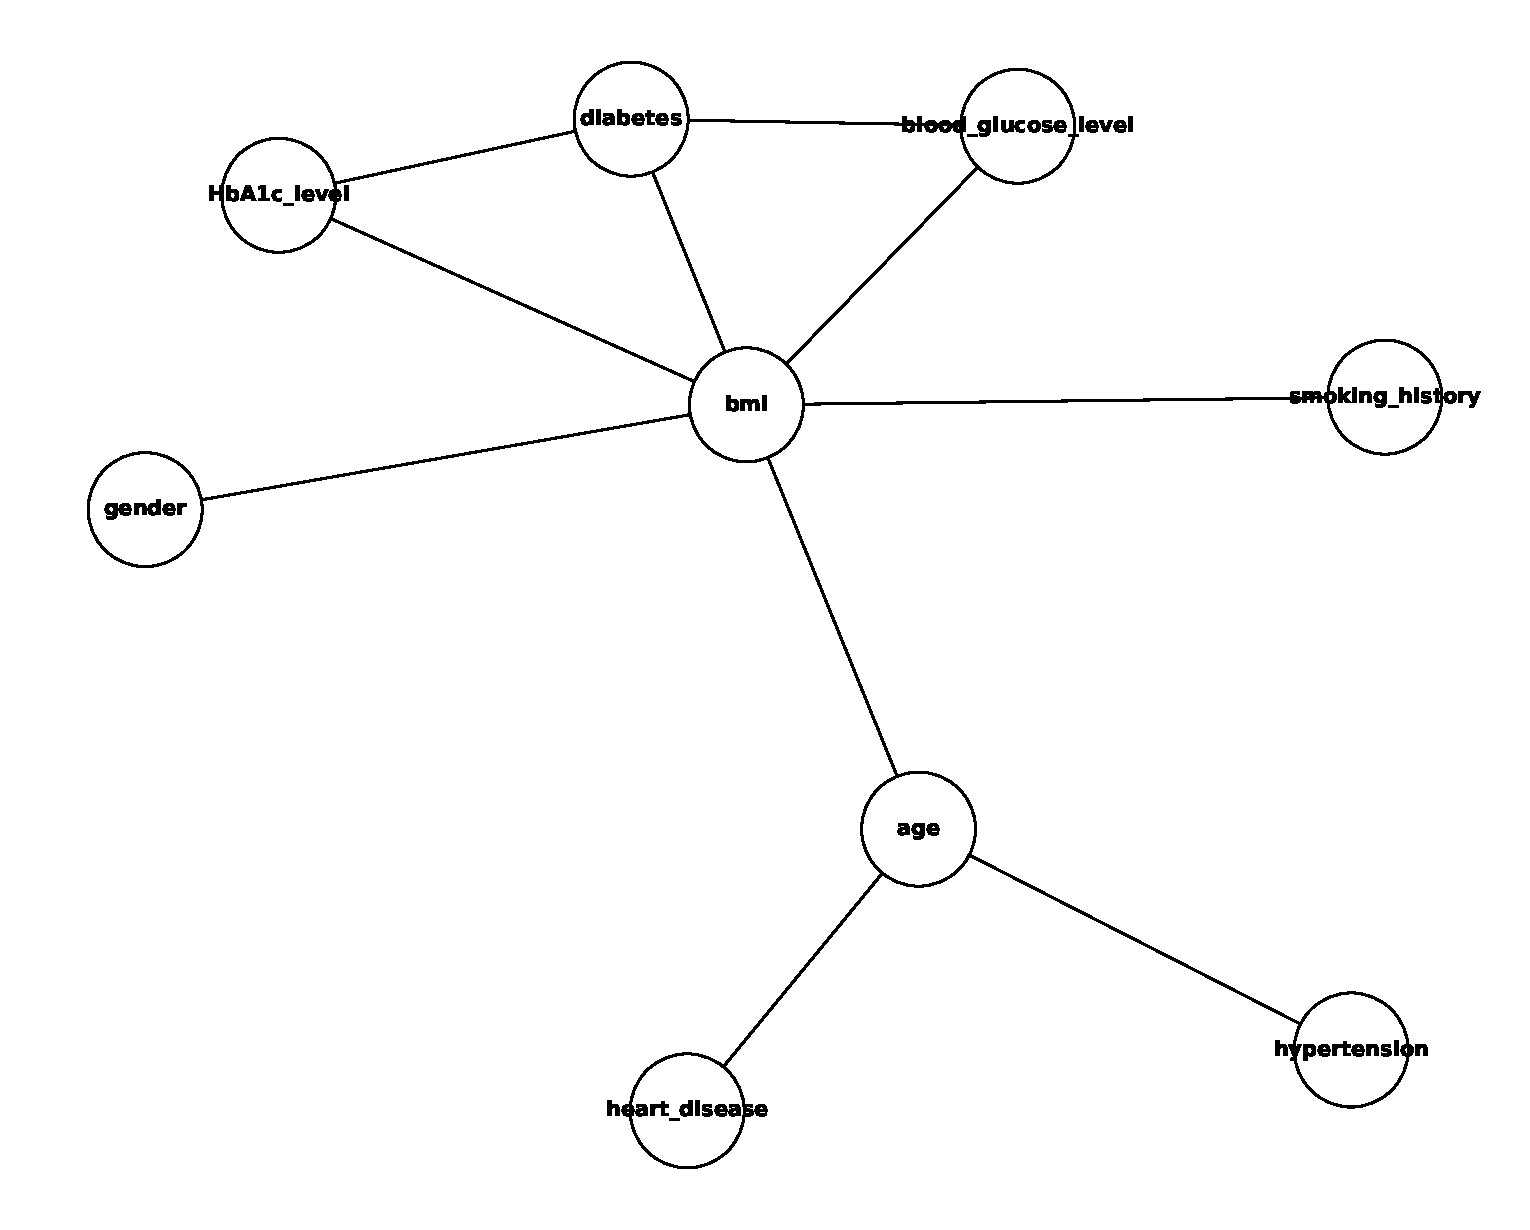
\includegraphics[width=\linewidth]{diabetes_mst}
\caption{Markov random field for marginals of the diabetes dataset.}
\label{fig:diabetes_mst}
\Description{Markov random field for marginals of the COMPAS dataset.}
\end{figure}

The same workflow was done as on previous datasets. The comparison results are shown in Table~\ref{tab:diabetes_score}.

There was also an increase of error on some sufficiency measure values. The sum of their differences is 0.189 and the average of their ratios is 0.489. However, this comparison may be skewed because one of the fairness measures in the original data was calculated to be zero, thus making the average ratio seem lower than otherwise.

\begin{table}[h]
\caption{Fairness measures experiment results of the COMPAS dataset. Sum of differences is 0.189. Average of ratios is 0.489.}
\label{tab:diabetes_score}
\begin{tabular}{ccccc}
\toprule
\textbf{Measure} & \textbf{Original} & \textbf{Synthetic} & \textbf{Diff} & \textbf{Ratio} \\
\midrule
Demographic Parity  & 0.013 & 0.015 & 0.002 & 0.867 \\
Accuracy Eqaulity   & 0.007 & 0.009 & 0.002 & 0.782 \\
Equalized Odds 1    & 0.000 & 0.003 & 0.003 & 0.000 \\
Equalized Odds 2    & 0.008 & 0.106 & 0.097 & 0.081 \\
Accuracy Equality 1 & 0.013 & 0.097 & 0.084 & 0.136 \\
Accuracy Equality 2 & 0.021 & 0.020 & 0.001 & 1.068 \\
\bottomrule
\end{tabular}
\end{table}

\section{Discussion}

\subsection{Accuracy}

\subsection{Impossibility}

\section{Conclusion}





%%
%% The acknowledgments section is defined using the "acks" environment
%% (and NOT an unnumbered section). This ensures the proper
%% identification of the section in the article metadata, and the
%% consistent spelling of the heading.
% \begin{acks}
% To Robert, for the bagels and explaining CMYK and color spaces.
% \end{acks}

%%
%% The next two lines define the bibliography style to be used, and
%% the bibliography file.
\bibliographystyle{ACM-Reference-Format}
\bibliography{references}


%%
%% If your work has an appendix, this is the place to put it.
% \appendix

\end{document}
\endinput
%%
%% End of file `sample-manuscript.tex'.
